\subsection{Fits\-Header  Class Reference}
\label{class_fitsheader}\index{FitsHeader@{Fits\-Header}}
Fits files and header keys. 


{\tt \#include $<$fitsimage.h$>$}

Inheritance diagram for Fits\-Header::\begin{figure}[H]
\begin{center}
\leavevmode
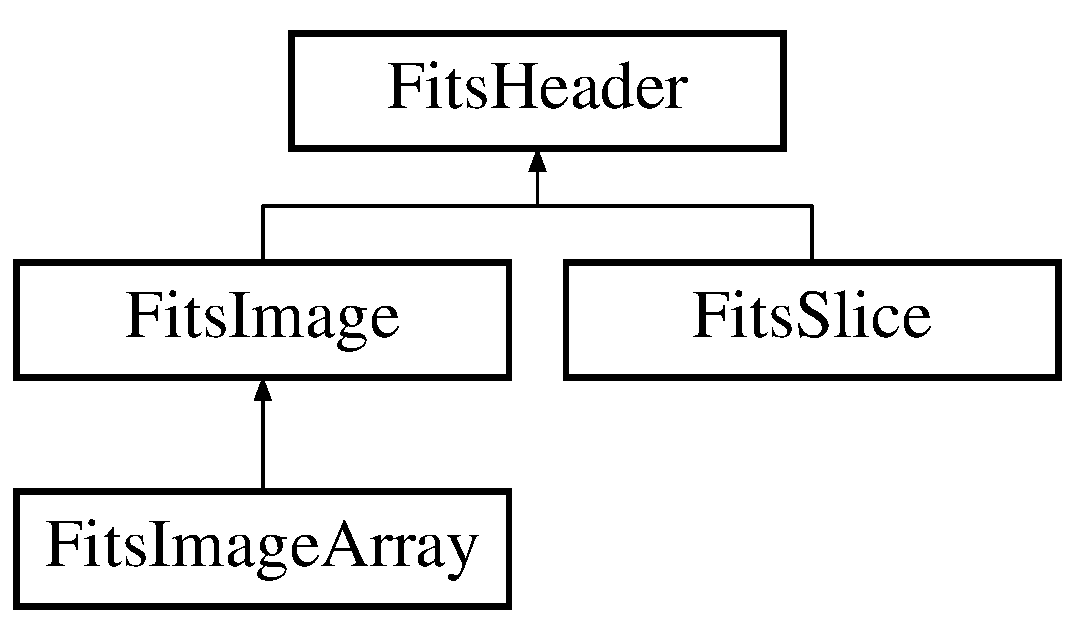
\includegraphics[height=3cm]{class_fitsheader}
\end{center}
\end{figure}
\subsubsection*{Public Methods}
\begin{CompactItemize}
\item 
\index{FitsHeader@{FitsHeader}!FitsHeader@{Fits\-Header}}\index{FitsHeader@{FitsHeader}!FitsHeader@{Fits\-Header}}
{\bf Fits\-Header} ()\label{class_fitsheader_a0}

\item 
\index{FitsHeader@{FitsHeader}!FitsHeader@{Fits\-Header}}\index{FitsHeader@{FitsHeader}!FitsHeader@{Fits\-Header}}
{\bf Fits\-Header} (const string \&File\-Name, const Fits\-File\-Mode Mode=RO, bool Empty\-File=false)\label{class_fitsheader_a1}

\begin{CompactList}\small\item\em opens the file, by default in readonly mode.\item\end{CompactList}\item 
\index{FitsHeader@{FitsHeader}!FitsHeader@{Fits\-Header}}\index{FitsHeader@{FitsHeader}!FitsHeader@{Fits\-Header}}
{\bf Fits\-Header} (const Fits\-Header \&a\_\-header, const string \&New\-File\-Name)\label{class_fitsheader_a2}

\begin{CompactList}\small\item\em opens a new file and copies a old header into it.\item\end{CompactList}\item 
\index{~FitsHeader@{$\sim$FitsHeader}!FitsHeader@{Fits\-Header}}\index{FitsHeader@{FitsHeader}!~FitsHeader@{$\sim$Fits\-Header}}
{\bf $\sim$Fits\-Header} ()\label{class_fitsheader_a3}

\item 
\index{IsValid@{IsValid}!FitsHeader@{Fits\-Header}}\index{FitsHeader@{FitsHeader}!IsValid@{Is\-Valid}}
bool {\bf Is\-Valid} () const\label{class_fitsheader_a4}

\begin{CompactList}\small\item\em returns if the file could be opened.\item\end{CompactList}\item 
\index{FileName@{FileName}!FitsHeader@{Fits\-Header}}\index{FitsHeader@{FitsHeader}!FileName@{File\-Name}}
string {\bf File\-Name} () const\label{class_fitsheader_a5}

\begin{CompactList}\small\item\em access routine to the fits file name.\item\end{CompactList}\item 
\index{FileMode@{FileMode}!FitsHeader@{Fits\-Header}}\index{FitsHeader@{FitsHeader}!FileMode@{File\-Mode}}
Fits\-File\-Mode {\bf File\-Mode} () const\label{class_fitsheader_a6}

\begin{CompactList}\small\item\em return the file mode (RO or RW).\item\end{CompactList}\item 
{\bf Fits\-Key} {\bf Key\-Val} (const string \&Key\-Name, const bool Warn=false) const
\begin{CompactList}\small\item\em read a key. warns on request.\item\end{CompactList}\item 
\index{KeyVal_Secure@{KeyVal\_\-Secure}!FitsHeader@{Fits\-Header}}\index{FitsHeader@{FitsHeader}!KeyVal_Secure@{Key\-Val\_\-Secure}}
{\bf Fits\-Key} {\bf Key\-Val\_\-Secure} (const string \&Key\-Name) const\label{class_fitsheader_a8}

\begin{CompactList}\small\item\em same above but test the presence of the key, and exit if not present.\item\end{CompactList}\item 
int {\bf Mod\-Key} (const string \&Key\-Name, const int Value, const string Comment=\char`\"{}\char`\"{}) const
\begin{CompactList}\small\item\em modifies an existing key value and comment.\item\end{CompactList}\item 
\index{ModKey@{ModKey}!FitsHeader@{Fits\-Header}}\index{FitsHeader@{FitsHeader}!ModKey@{Mod\-Key}}
int {\bf Mod\-Key} (const string \&Key\-Name, const double Value, const string Comment=\char`\"{}\char`\"{}) const\label{class_fitsheader_a10}

\begin{CompactList}\small\item\em -.\item\end{CompactList}\item 
\index{ModKey@{ModKey}!FitsHeader@{Fits\-Header}}\index{FitsHeader@{FitsHeader}!ModKey@{Mod\-Key}}
int {\bf Mod\-Key} (const string \&Key\-Name, const char $\ast$Value, const string Comment=\char`\"{}\char`\"{}) const\label{class_fitsheader_a11}

\begin{CompactList}\small\item\em -.\item\end{CompactList}\item 
\index{ModKey@{ModKey}!FitsHeader@{Fits\-Header}}\index{FitsHeader@{FitsHeader}!ModKey@{Mod\-Key}}
int {\bf Mod\-Key} (const string \&Key\-Name, const bool Value, const string Comment=\char`\"{}\char`\"{}) const\label{class_fitsheader_a12}

\begin{CompactList}\small\item\em -.\item\end{CompactList}\item 
int {\bf Add\-Key} (const string \&Key\-Name, const char $\ast$Key\-Val, const string Comment=\char`\"{}\char`\"{})
\begin{CompactList}\small\item\em adds (at the end of the header) a new key.\item\end{CompactList}\item 
\index{AddKey@{AddKey}!FitsHeader@{Fits\-Header}}\index{FitsHeader@{FitsHeader}!AddKey@{Add\-Key}}
int {\bf Add\-Key} (const string \&Key\-Name, const double Key\-Val, const string Comment=\char`\"{}\char`\"{})\label{class_fitsheader_a14}

\item 
\index{AddKey@{AddKey}!FitsHeader@{Fits\-Header}}\index{FitsHeader@{FitsHeader}!AddKey@{Add\-Key}}
int {\bf Add\-Key} (const string \&Key\-Name, const int Key\-Val, const string Comment=\char`\"{}\char`\"{})\label{class_fitsheader_a15}

\item 
\index{AddKey@{AddKey}!FitsHeader@{Fits\-Header}}\index{FitsHeader@{FitsHeader}!AddKey@{Add\-Key}}
int {\bf Add\-Key} (const string \&Key\-Name, const bool Key\-Val, const string Comment=\char`\"{}\char`\"{})\label{class_fitsheader_a16}

\item 
\index{AddOrModKey@{AddOrModKey}!FitsHeader@{Fits\-Header}}\index{FitsHeader@{FitsHeader}!AddOrModKey@{Add\-Or\-Mod\-Key}}
int {\bf Add\-Or\-Mod\-Key} (const string \&Key\-Name, const char $\ast$Value, const string Comment=\char`\"{}\char`\"{})\label{class_fitsheader_a17}

\begin{CompactList}\small\item\em modifies an existing key or adds it if it does not exist yet.\item\end{CompactList}\item 
\index{AddOrModKey@{AddOrModKey}!FitsHeader@{Fits\-Header}}\index{FitsHeader@{FitsHeader}!AddOrModKey@{Add\-Or\-Mod\-Key}}
int {\bf Add\-Or\-Mod\-Key} (const string \&Key\-Name, const string \&Value, const string Comment=\char`\"{}\char`\"{})\label{class_fitsheader_a18}

\begin{CompactList}\small\item\em modifies an existing key or adds it if it does not exist yet.\item\end{CompactList}\item 
\index{AddOrModKey@{AddOrModKey}!FitsHeader@{Fits\-Header}}\index{FitsHeader@{FitsHeader}!AddOrModKey@{Add\-Or\-Mod\-Key}}
int {\bf Add\-Or\-Mod\-Key} (const string \&Key\-Name, const double Value, const string Comment=\char`\"{}\char`\"{})\label{class_fitsheader_a19}

\begin{CompactList}\small\item\em modifies an existing key or adds it if it does not exist yet.\item\end{CompactList}\item 
\index{AddOrModKey@{AddOrModKey}!FitsHeader@{Fits\-Header}}\index{FitsHeader@{FitsHeader}!AddOrModKey@{Add\-Or\-Mod\-Key}}
int {\bf Add\-Or\-Mod\-Key} (const string \&Key\-Name, const int Value, const string Comment=\char`\"{}\char`\"{})\label{class_fitsheader_a20}

\begin{CompactList}\small\item\em modifies an existing key or adds it if it does not exist yet.\item\end{CompactList}\item 
\index{AddOrModKey@{AddOrModKey}!FitsHeader@{Fits\-Header}}\index{FitsHeader@{FitsHeader}!AddOrModKey@{Add\-Or\-Mod\-Key}}
int {\bf Add\-Or\-Mod\-Key} (const string \&Key\-Name, const bool Value, const string Comment=\char`\"{}\char`\"{})\label{class_fitsheader_a21}

\begin{CompactList}\small\item\em modifies an existing key or adds it if it does not exist yet.\item\end{CompactList}\item 
int {\bf Key\-Match} (const string \&Key\-Pattern, Fits\-Key\-Array \&Array) const
\begin{CompactList}\small\item\em To read keys following a pattern.\item\end{CompactList}\item 
\index{ModKeyName@{ModKeyName}!FitsHeader@{Fits\-Header}}\index{FitsHeader@{FitsHeader}!ModKeyName@{Mod\-Key\-Name}}
int {\bf Mod\-Key\-Name} (const string \&Old\-Key\-Name, const string \&New\-Key\-Name) const\label{class_fitsheader_a23}

\begin{CompactList}\small\item\em changes the Key itself.\item\end{CompactList}\item 
\index{ModKeyComment@{ModKeyComment}!FitsHeader@{Fits\-Header}}\index{FitsHeader@{FitsHeader}!ModKeyComment@{Mod\-Key\-Comment}}
int {\bf Mod\-Key\-Comment} (const string \&Key\-Name, const string \&New\-Comment) const\label{class_fitsheader_a24}

\begin{CompactList}\small\item\em changes the comment.\item\end{CompactList}\item 
\index{HasKey@{HasKey}!FitsHeader@{Fits\-Header}}\index{FitsHeader@{FitsHeader}!HasKey@{Has\-Key}}
bool {\bf Has\-Key} (const string \&Key\-Name, const bool Warn=false) const\label{class_fitsheader_a25}

\begin{CompactList}\small\item\em enables to check the presence of a key. warns on request.\item\end{CompactList}\item 
\index{HasActualKey@{HasActualKey}!FitsHeader@{Fits\-Header}}\index{FitsHeader@{FitsHeader}!HasActualKey@{Has\-Actual\-Key}}
bool {\bf Has\-Actual\-Key} (const string \&Key\-Name, const bool Warn=false) const\label{class_fitsheader_a26}

\begin{CompactList}\small\item\em has a genuine fits key.\item\end{CompactList}\item 
\index{RmKey@{RmKey}!FitsHeader@{Fits\-Header}}\index{FitsHeader@{FitsHeader}!RmKey@{Rm\-Key}}
int {\bf Rm\-Key} (const string \&Key\-Name) const\label{class_fitsheader_a27}

\begin{CompactList}\small\item\em deletes a key.\item\end{CompactList}\item 
\index{NKeys@{NKeys}!FitsHeader@{Fits\-Header}}\index{FitsHeader@{FitsHeader}!NKeys@{NKeys}}
int {\bf NKeys} () const\label{class_fitsheader_a28}

\begin{CompactList}\small\item\em return the number of keys (without counting the END key).\item\end{CompactList}\item 
\index{CopyKey@{CopyKey}!FitsHeader@{Fits\-Header}}\index{FitsHeader@{FitsHeader}!CopyKey@{Copy\-Key}}
bool {\bf Copy\-Key} (const char $\ast$Key\-Name, Fits\-Header \&To) const\label{class_fitsheader_a29}

\begin{CompactList}\small\item\em copy verbatim a key (name, value, comment).\item\end{CompactList}\item 
int {\bf Add\-Comment\-Line} (const string \&AVery\-Useful\-Comment)
\begin{CompactList}\small\item\em add a COMMENT keyword.\item\end{CompactList}\item 
int {\bf Add\-History\-Line} (const string \&History\-Stuff)
\begin{CompactList}\small\item\em add a HISTORY keyword.\item\end{CompactList}\item 
\index{Flush@{Flush}!FitsHeader@{Fits\-Header}}\index{FitsHeader@{FitsHeader}!Flush@{Flush}}
int {\bf Flush} ()\label{class_fitsheader_a32}

\begin{CompactList}\small\item\em flush file buffers.\item\end{CompactList}\item 
\index{AddOrModCard@{AddOrModCard}!FitsHeader@{Fits\-Header}}\index{FitsHeader@{FitsHeader}!AddOrModCard@{Add\-Or\-Mod\-Card}}
int {\bf Add\-Or\-Mod\-Card} (const string \&Key\-Name, const string \&Card)\label{class_fitsheader_a33}

\begin{CompactList}\small\item\em add a whole card, name+value+comment (or modifies an existing one).\item\end{CompactList}\item 
\index{ImageSizes@{ImageSizes}!FitsHeader@{Fits\-Header}}\index{FitsHeader@{FitsHeader}!ImageSizes@{Image\-Sizes}}
void {\bf Image\-Sizes} (int \&Xsize, int \&YSize) const\label{class_fitsheader_a34}

\item 
\index{SameImageSizes@{SameImageSizes}!FitsHeader@{Fits\-Header}}\index{FitsHeader@{FitsHeader}!SameImageSizes@{Same\-Image\-Sizes}}
bool {\bf Same\-Image\-Sizes} (const Fits\-Header \&Other) const\label{class_fitsheader_a35}

\item 
\index{ImageCenter@{ImageCenter}!FitsHeader@{Fits\-Header}}\index{FitsHeader@{FitsHeader}!ImageCenter@{Image\-Center}}
{\bf Point} {\bf Image\-Center} () const\label{class_fitsheader_a36}

\begin{CompactList}\small\item\em The geometric center of the image.\item\end{CompactList}\item 
\index{SameChipFilterInst@{SameChipFilterInst}!FitsHeader@{Fits\-Header}}\index{FitsHeader@{FitsHeader}!SameChipFilterInst@{Same\-Chip\-Filter\-Inst}}
bool {\bf Same\-Chip\-Filter\-Inst} (const Fits\-Header \&Other, const bool Warn=true) const\label{class_fitsheader_a37}

\begin{CompactList}\small\item\em checks that both images refer to the same chip, filter and instrument.\item\end{CompactList}\item 
\index{SameChipFilter@{SameChipFilter}!FitsHeader@{Fits\-Header}}\index{FitsHeader@{FitsHeader}!SameChipFilter@{Same\-Chip\-Filter}}
bool {\bf Same\-Chip\-Filter} (const Fits\-Header \&Other, const bool Warn=true) const\label{class_fitsheader_a38}

\begin{CompactList}\small\item\em checks that both images refer to the same chip and filter.\item\end{CompactList}\item 
\index{SameChipFilter@{SameChipFilter}!FitsHeader@{Fits\-Header}}\index{FitsHeader@{FitsHeader}!SameChipFilter@{Same\-Chip\-Filter}}
bool {\bf Same\-Chip\-Filter} (const string \&Other\-Fits\-Name, const bool Warn=true) const\label{class_fitsheader_a39}

\item 
\index{SameFilter@{SameFilter}!FitsHeader@{Fits\-Header}}\index{FitsHeader@{FitsHeader}!SameFilter@{Same\-Filter}}
bool {\bf Same\-Filter} (const Fits\-Header \&Other, const bool Warn=true) const\label{class_fitsheader_a40}

\begin{CompactList}\small\item\em checks that both images refer to the same filter.\item\end{CompactList}\item 
\index{SameFilter@{SameFilter}!FitsHeader@{Fits\-Header}}\index{FitsHeader@{FitsHeader}!SameFilter@{Same\-Filter}}
bool {\bf Same\-Filter} (const string \&Other\-Fits\-Name, const bool Warn=true) const\label{class_fitsheader_a41}

\item 
\index{SameChip@{SameChip}!FitsHeader@{Fits\-Header}}\index{FitsHeader@{FitsHeader}!SameChip@{Same\-Chip}}
bool {\bf Same\-Chip} (const Fits\-Header \&Other, const bool Warn=true) const\label{class_fitsheader_a42}

\begin{CompactList}\small\item\em checks that both images refer to the same chip.\item\end{CompactList}\item 
\index{SameChip@{SameChip}!FitsHeader@{Fits\-Header}}\index{FitsHeader@{FitsHeader}!SameChip@{Same\-Chip}}
bool {\bf Same\-Chip} (const string \&Other\-Fits\-Name, const bool Warn=true) const\label{class_fitsheader_a43}

\begin{CompactList}\small\item\em same as above, using file name.\item\end{CompactList}\item 
\index{TelInst@{TelInst}!FitsHeader@{Fits\-Header}}\index{FitsHeader@{FitsHeader}!TelInst@{Tel\-Inst}}
Virtual\-Instrument$\ast$ {\bf Tel\-Inst} () const\label{class_fitsheader_a44}

\item 
void {\bf Enable\-Write} (const bool Yes\-Or\-No)
\begin{CompactList}\small\item\em for a {\bf Fits\-Image} {\rm (p.\,\pageref{class_fitsimage})} opened RW, enables to forbid writing (default behaviour) when destructor is called.\item\end{CompactList}\item 
\index{FitsHeader@{FitsHeader}!FitsHeader@{Fits\-Header}}\index{FitsHeader@{FitsHeader}!FitsHeader@{Fits\-Header}}
{\bf Fits\-Header} (const Fits\-Header \&)\label{class_fitsheader_a46}

\item 
\index{Append_LowPriority@{Append\_\-LowPriority}!FitsHeader@{Fits\-Header}}\index{FitsHeader@{FitsHeader}!Append_LowPriority@{Append\_\-Low\-Priority}}
void {\bf Append\_\-Low\-Priority} (const Fits\-Header \&To\-Append)\label{class_fitsheader_a47}

\item 
\index{MoveHDU@{MoveHDU}!FitsHeader@{Fits\-Header}}\index{FitsHeader@{FitsHeader}!MoveHDU@{Move\-HDU}}
int {\bf Move\-HDU} (int How\-Many=1)\label{class_fitsheader_a48}

\item 
\index{CopyCHDUTo@{CopyCHDUTo}!FitsHeader@{Fits\-Header}}\index{FitsHeader@{FitsHeader}!CopyCHDUTo@{Copy\-CHDUTo}}
int {\bf Copy\-CHDUTo} (Fits\-Header \&Out\-Header)\label{class_fitsheader_a49}

\item 
\index{CopyDataTo@{CopyDataTo}!FitsHeader@{Fits\-Header}}\index{FitsHeader@{FitsHeader}!CopyDataTo@{Copy\-Data\-To}}
int {\bf Copy\-Data\-To} (Fits\-Header \&Out\-Header)\label{class_fitsheader_a50}

\item 
\index{NHDU@{NHDU}!FitsHeader@{Fits\-Header}}\index{FitsHeader@{FitsHeader}!NHDU@{NHDU}}
int {\bf NHDU} () const\label{class_fitsheader_a51}

\end{CompactItemize}
\subsubsection*{Friends}
\begin{CompactItemize}
\item 
class {\bf Fits\-Image\-Array}
\item 
class {\bf Fits\-Key}
\item 
class {\bf Fits\-Image}
\item 
class {\bf Fits\-Slice}
\item 
\index{operator<<@{operator$<$$<$}!FitsHeader@{Fits\-Header}}\index{FitsHeader@{FitsHeader}!operator<<@{operator$<$$<$}}
ostream\& {\bf operator$<$$<$} (ostream \&stream, const Fits\-Header \&Header)\label{class_fitsheader_l4}

\begin{CompactList}\small\item\em enables : \footnotesize\begin{verbatim} cout << FitsHeader("my_image.fits"); \end{verbatim}\normalsize 
.\item\end{CompactList}\end{CompactItemize}


\subsubsection{Detailed Description}
Fits files and header keys.

The Fits\-Header class does not deal with the data part of fits files. The actual engine is cfitsio. 



\subsubsection{Member Function Documentation}
\index{FitsHeader@{Fits\-Header}!AddCommentLine@{AddCommentLine}}
\index{AddCommentLine@{AddCommentLine}!FitsHeader@{Fits\-Header}}
\paragraph{\setlength{\rightskip}{0pt plus 5cm}int Fits\-Header::Add\-Comment\-Line (const string \& {\em AVery\-Useful\-Comment})}\hfill\label{class_fitsheader_a30}


add a COMMENT keyword.

It will be split over multiple  COMMENT lines if longer than 70 characters. \index{FitsHeader@{Fits\-Header}!AddHistoryLine@{AddHistoryLine}}
\index{AddHistoryLine@{AddHistoryLine}!FitsHeader@{Fits\-Header}}
\paragraph{\setlength{\rightskip}{0pt plus 5cm}int Fits\-Header::Add\-History\-Line (const string \& {\em History\-Stuff})}\hfill\label{class_fitsheader_a31}


add a HISTORY keyword.

It will be split over multiple  HISTORY lines if longer than 70 characters. \index{FitsHeader@{Fits\-Header}!AddKey@{AddKey}}
\index{AddKey@{AddKey}!FitsHeader@{Fits\-Header}}
\paragraph{\setlength{\rightskip}{0pt plus 5cm}int Fits\-Header::Add\-Key (const string \& {\em Key\-Name}, const char $\ast$ {\em Key\-Val}, const string {\em Comment} = \char`\"{}\char`\"{})}\hfill\label{class_fitsheader_a13}


adds (at the end of the header) a new key.

Checks before that this key does not exist yet. No comment if Comment is NULL or absent. Value can be int, double, char$\ast$, or bool. \index{FitsHeader@{Fits\-Header}!EnableWrite@{EnableWrite}}
\index{EnableWrite@{EnableWrite}!FitsHeader@{Fits\-Header}}
\paragraph{\setlength{\rightskip}{0pt plus 5cm}void Fits\-Header::Enable\-Write (const bool {\em Yes\-Or\-No})}\hfill\label{class_fitsheader_a45}


for a {\bf Fits\-Image} {\rm (p.\,\pageref{class_fitsimage})} opened RW, enables to forbid writing (default behaviour) when destructor is called.

example of use : the flatfielding opens (RW) the flatfielded {\bf Fits\-Image} {\rm (p.\,\pageref{class_fitsimage})}, and  only allow writing on successful flatfielding completion. \index{FitsHeader@{Fits\-Header}!KeyMatch@{KeyMatch}}
\index{KeyMatch@{KeyMatch}!FitsHeader@{Fits\-Header}}
\paragraph{\setlength{\rightskip}{0pt plus 5cm}int Fits\-Header::Key\-Match (const string \& {\em Key\-Pattern}, Fits\-Key\-Array \& {\em Array}) const}\hfill\label{class_fitsheader_a22}


To read keys following a pattern.

$\ast$ matches anything, ? a single character, \# successive decimal digits. Array[i]. size() returns the number of matched keys. Array[i].Key\-Name and \{double,string,int\}(Array[i]) enable to accees  key names and values \index{FitsHeader@{Fits\-Header}!KeyVal@{KeyVal}}
\index{KeyVal@{KeyVal}!FitsHeader@{Fits\-Header}}
\paragraph{\setlength{\rightskip}{0pt plus 5cm}{\bf Fits\-Key} Fits\-Header::Key\-Val (const string \& {\em Key\-Name}, const bool {\em Warn} = false) const}\hfill\label{class_fitsheader_a7}


read a key. warns on request.

use (e.g.) \footnotesize\begin{verbatim} double ra = a_header.KeyVal("RA"); \end{verbatim}\normalsize 
 adequate converters are applied for int, double, float, string and bool variables. \index{FitsHeader@{Fits\-Header}!ModKey@{ModKey}}
\index{ModKey@{ModKey}!FitsHeader@{Fits\-Header}}
\paragraph{\setlength{\rightskip}{0pt plus 5cm}int Fits\-Header::Mod\-Key (const string \& {\em Key\-Name}, const int {\em Value}, const string {\em Comment} = \char`\"{}\char`\"{}) const}\hfill\label{class_fitsheader_a9}


modifies an existing key value and comment.

If comment is NULL the comment is unchanged. 

The documentation for this class was generated from the following file:\begin{CompactItemize}
\item 
{\bf fitsimage.h}\end{CompactItemize}
